
% LaTeX-Vorlage für Versuchsprotokolle
% Autor: Simon May
% Datum: 2017-10-05

% Es gibt die Dokumenttypen scrartcl („Artikel“), scrreprt („Bericht“),
% scrbook („Buch“) und scrlttr2 („Brief“). Diese gehören zum KOMA-Script,
% bieten mehr Optionen als die „Standardklassen“ und sollten besonders für
% deutsche Texte benutzt werden.
% Natürlich gibt es noch weitere Klassen, z.B. beamer für Präsentationen.
\documentclass[
	a4paper,                % Papierformat (DIN A4)
	titlepage=firstiscover, % Separate Titelseite
	captions=tableheading,  % \caption bei Tabellen immer als Überschrift setzen
	toc=bibliography,       % Literaturverzeichnis im Inhaltsverzeichnis aufführen
	toc=listof,             % Abbildungsverzeichnis etc. im Inhaltsverzeichnis aufführen
	oneside,                % Einseitig
	%twoside,               % Zweiseitig
	%twocolumn,             % Zweispaltig
	automark,               % Abschnittstitel automatisch in Kopfzeile einfügen
	12pt,                   % Schriftgröße (beliebige Größen mit „fontsize=Xpt“)
	english, ngerman,       % Sprache für z.B. Babel; ausgewählt: ngerman (letztgenannt)
	%draft=true             % Entwurf-Modus; markiert zu lange und zu kurze Zeilen
]{scrartcl}

% --- Pakete einbinden
% Autor: Simon May
% Datum: 2017-10-04

% --- Pakete einbinden
% --- Pakete erweitern LaTeX um zusätzliche Funktionen.
%     Dies ist ein Satz nützlicher Pakete.

% Silbentrennung etc.; Sprache wird durch Option bei \documentclass festgelegt
\usepackage{babel}
\usepackage{iftex}
\ifLuaTeX
	% Schriftart (Latin Modern)
	\usepackage{fontspec}
	\fontspec{Latin Modern Roman}
\else
	% Verwendung der Zeichentabelle T1 (für Sonderzeichen etc.)
	\usepackage[T1]{fontenc}
	% Legt die Eingabe-Zeichenkodierung fest, z.B. UTF-8
	\usepackage[utf8]{inputenc}
	% Schriftart (Latin Modern)
	\usepackage{lmodern}
	% Zusätzliche Sonderzeichen
	\usepackage{textcomp}
\fi

% Nutzen von +, -, *, / in \setlength u.ä. (z.B. \setlength{\a + 3cm})
\usepackage{calc}
% Wird benötigt, um \ifthenelse zu benutzen
\usepackage{xifthen}
% Optionen für eigene definierte Befehle
\usepackage{xparse}

% Verbessertes Aussehen des Schriftbilds durch kleine Anpassungen
\usepackage{microtype}
% Automatische Formatierung von Daten
\usepackage[useregional]{datetime2}
% Wird für Kopf- und Fußzeile benötigt
\usepackage{scrlayer-scrpage}
% Einfaches Wechseln zwischen unterschiedlichen Zeilenabständen
\usepackage{setspace}
% Optionen für Listen (enumerate, itemize, …)
\usepackage{enumitem}
% Automatische Anführungszeichen
\usepackage{csquotes}
% Zusätzliche Optionen für Tabellen (tabular)
\usepackage{array}

% Mathepaket (intlimits: Grenzen über/unter Integralzeichen)
\usepackage[intlimits]{amsmath}
% Mathe-Symbole, \mathbb etc.
\usepackage{amssymb}
% Weitere Mathebefehle
\usepackage{mathtools}
% „Schöne“ Brüche im Fließtext
\usepackage{xfrac}
% Ermöglicht die Nutzung von \SI{Zahl}{Einheit} u.a.
\usepackage{siunitx}
% Definition von Unicode-Symbolen; Nach [utf8]inputenc laden!
\usepackage{newunicodechar}
% Unicode-Formeln mit pdfLaTeX
% Autor: Simon May
% Datum: 2015-03-04

% Diese Datei ermöglicht es, Mathe-Symbole (z.B. \gamma) direkt als
% Sonderzeichen (d.h. γ) einzugeben

% silence unterdrückt Warnungen; vor hyperref laden
\usepackage{silence}
\WarningFilter[pdflatex-unicode-math]{newunicodechar}{Redefining Unicode character}
\ActivateWarningFilters[pdflatex-unicode-math]

\newunicodechar{†}{\dag}
\newunicodechar{‡}{\ddag}
\newunicodechar{…}{\ldots}
\newunicodechar{⋯}{\cdots}
\newunicodechar{⋮}{\vdots}
\newunicodechar{⋱}{\ddots}
\newunicodechar{⋰}{\iddots}
\newunicodechar{α}{\alpha}
\newunicodechar{β}{\beta}
\newunicodechar{γ}{\gamma}
\newunicodechar{δ}{\delta}
\newunicodechar{ε}{\varepsilon}
\newunicodechar{ϵ}{\epsilon}
\newunicodechar{ζ}{\zeta}
\newunicodechar{η}{\eta}
\newunicodechar{θ}{\theta}
\newunicodechar{ϑ}{\vartheta}
\newunicodechar{ι}{\iota}
\newunicodechar{κ}{\kappa}
\newunicodechar{ϰ}{\varkappa}
\newunicodechar{λ}{\lambda}
\newunicodechar{μ}{\mu}
\newunicodechar{ν}{\nu}
\newunicodechar{ξ}{\xi}
\newunicodechar{ο}{o}
\newunicodechar{π}{\pi}
\newunicodechar{ρ}{\rho}
\newunicodechar{ϱ}{\varrho}
\newunicodechar{σ}{\sigma}
\newunicodechar{τ}{\tau}
\newunicodechar{υ}{\upsilon}
\newunicodechar{φ}{\varphi}
\newunicodechar{ϕ}{\phi}
\newunicodechar{χ}{\chi}
\newunicodechar{ψ}{\psi}
\newunicodechar{ω}{\omega}
\newunicodechar{Α}{\mathrm{A}}
\newunicodechar{Β}{\mathrm{B}}
\newunicodechar{Γ}{\Gamma}
\newunicodechar{Δ}{\Delta}
\newunicodechar{Ε}{\mathrm{E}}
\newunicodechar{Ζ}{\mathrm{Z}}
\newunicodechar{Η}{\mathrm{H}}
\newunicodechar{Θ}{\Theta}
\newunicodechar{Ι}{\mathrm{I}}
\newunicodechar{Κ}{\mathrm{K}}
\newunicodechar{Λ}{\Lambda}
\newunicodechar{Μ}{\mathrm{M}}
\newunicodechar{Ν}{\mathrm{N}}
\newunicodechar{Ξ}{\Xi}
\newunicodechar{Ο}{\mathrm{O}}
\newunicodechar{Π}{\Pi}
\newunicodechar{Ρ}{\mathrm{P}}
\newunicodechar{Σ}{\Sigma}
\newunicodechar{Τ}{\mathrm{T}}
\newunicodechar{Υ}{\Upsilon}
\newunicodechar{Φ}{\Phi}
\newunicodechar{Χ}{\Chi}
\newunicodechar{Ψ}{\Psi}
\newunicodechar{Ω}{\Omega}
\newunicodechar{∑}{\sum}
\newunicodechar{∫}{\int}
\newunicodechar{∬}{\iint}
\newunicodechar{∭}{\iiint}
\newunicodechar{⨌}{\iiiint}
\newunicodechar{∮}{\oint}
\newunicodechar{∯}{\oiint}
\newunicodechar{∰}{\oiiint}
\newunicodechar{∇}{\nabla}
\newunicodechar{∂}{\partial}
\newunicodechar{√}{\sqrt}
\newunicodechar{∈}{\in}
\newunicodechar{∋}{\ni}
\newunicodechar{∉}{\notin}
\newunicodechar{∀}{\forall}
\newunicodechar{∃}{\exists}
\newunicodechar{∄}{\nexists}
\newunicodechar{∴}{\therefore}
\newunicodechar{∵}{\because}
\newunicodechar{〈}{\langle}
\newunicodechar{〉}{\rangle}
\newunicodechar{⌊}{\lfloor}
\newunicodechar{⌋}{\rfloor}
\newunicodechar{⌈}{\lceil}
\newunicodechar{⌉}{\rceil}
\newunicodechar{∼}{\sim}
\newunicodechar{∝}{\propto}
\newunicodechar{∞}{\infty}
\newunicodechar{ℵ}{\aleph}
\newunicodechar{ℏ}{\hbar}
\newunicodechar{℘}{\wp}
\newunicodechar{ℓ}{\ell}
\newunicodechar{∅}{\emptyset}
\newunicodechar{×}{\times}
\newunicodechar{⋅}{\cdot}
\newunicodechar{÷}{\div}
\newunicodechar{⋆}{\star}
\newunicodechar{∘}{\circ}
\newunicodechar{⋄}{\diamond}
\newunicodechar{⊕}{\oplus}
\newunicodechar{⊖}{\ominus}
\newunicodechar{⊗}{\otimes}
\newunicodechar{⊘}{\oslash}
\newunicodechar{⊙}{\odot}
\newunicodechar{±}{\pm}
\newunicodechar{∓}{\mp}
\newunicodechar{≈}{\approx}
\newunicodechar{≡}{\equiv}
\newunicodechar{≠}{\ne}
\newunicodechar{≥}{\ge}
\newunicodechar{≤}{\le}
\newunicodechar{≫}{\gg}
\newunicodechar{≪}{\ll}
\newunicodechar{⊂}{\subset}
\newunicodechar{⊃}{\supset}
\newunicodechar{⊆}{\subseteq}
\newunicodechar{⊇}{\supseteq}
\newunicodechar{⊈}{\nsubseteq}
\newunicodechar{⊉}{\nsupseteq}
\newunicodechar{≔}{\coloneqq}
\newunicodechar{≕}{\eqqcolon}
\newunicodechar{¬}{\neg}
\newunicodechar{∨}{\vee}
\newunicodechar{∧}{\wedge}
\newunicodechar{∪}{\cup}
\newunicodechar{∩}{\cap}
\newunicodechar{⋁}{\bigvee}
\newunicodechar{⋀}{\bigwedge}
\newunicodechar{⋃}{\bigcup}
\newunicodechar{⋂}{\bigcap}
\newunicodechar{⟂}{\perp}
\newunicodechar{∥}{\parallel}
\newunicodechar{∦}{\nparallel}
\newunicodechar{𝚤}{\imath}
\newunicodechar{𝚥}{\jmath}
\newunicodechar{⇔}{\Leftrightarrow}
\newunicodechar{⇕}{\Updownarrow}
\newunicodechar{⇐}{\Leftarrow}
\newunicodechar{⇒}{\Rightarrow}
\newunicodechar{⇑}{\Uparrow}
\newunicodechar{⇓}{\Downarrow}
\newunicodechar{↔}{\leftrightarrow}
\newunicodechar{↕}{\updownarrow}
\newunicodechar{←}{\leftarrow}
\newunicodechar{→}{\rightarrow}
\newunicodechar{↑}{\uparrow}
\newunicodechar{↓}{\downarrow}
\newunicodechar{⟷}{\longleftrightarrow}
\newunicodechar{⟵}{\longleftarrow}
\newunicodechar{⟶}{\longrightarrow}
\newunicodechar{⇇}{\leftleftarrows}
\newunicodechar{⇉}{\rightrightarrows}
\newunicodechar{⇈}{\upuparrows}
\newunicodechar{⇊}{\downdownarrows}
\newunicodechar{⟺}{\Longleftrightarrow}
\newunicodechar{⟸}{\Longleftarrow}
\newunicodechar{⟹}{\Longrightarrow}
\newunicodechar{↦}{\mapsto}
\newunicodechar{↤}{\mapsfrom}
\newunicodechar{⟼}{\longmapsto}
\newunicodechar{⟻}{\longmapsfrom}
\newunicodechar{⟾}{\Longmapsto}
\newunicodechar{⟽}{\Longmapsfrom}
\newunicodechar{↗}{\nearrow}
\newunicodechar{↖}{\nwarrow}
\newunicodechar{↘}{\searrow}
\newunicodechar{↙}{\swarrow}
\newunicodechar{↩}{\hookleftarrow}
\newunicodechar{↪}{\hookrightarrow}
\newunicodechar{↶}{\curvearrowleft}
\newunicodechar{↷}{\curvearrowright}
\newunicodechar{↺}{\circlearrowleft}
\newunicodechar{↻}{\circlearrowright}
\newunicodechar{↫}{\looparrowleft}
\newunicodechar{↬}{\looparrowright}
\newunicodechar{⇋}{\leftrightharpoons}
\newunicodechar{⇌}{\rightleftharpoons}
\newunicodechar{↼}{\leftharpoonup}
\newunicodechar{↽}{\leftharpoondown}
\newunicodechar{⇀}{\rightharpoonup}
\newunicodechar{⇁}{\rightharpoondown}
\newunicodechar{↿}{\upharpoonleft}
\newunicodechar{↾}{\upharpoonright}
\newunicodechar{⇃}{\downharpoonleft}
\newunicodechar{⇂}{\downharpoonright}
\newunicodechar{𝔸}{\mathbb{A}}
\newunicodechar{𝔹}{\mathbb{B}}
\newunicodechar{ℂ}{\mathbb{C}}
\newunicodechar{𝔻}{\mathbb{D}}
\newunicodechar{𝔼}{\mathbb{E}}
\newunicodechar{𝔽}{\mathbb{F}}
\newunicodechar{𝔾}{\mathbb{G}}
\newunicodechar{ℍ}{\mathbb{H}}
\newunicodechar{𝕀}{\mathbb{I}}
\newunicodechar{𝕁}{\mathbb{J}}
\newunicodechar{𝕂}{\mathbb{K}}
\newunicodechar{𝕃}{\mathbb{L}}
\newunicodechar{𝕄}{\mathbb{M}}
\newunicodechar{ℕ}{\mathbb{N}}
\newunicodechar{𝕆}{\mathbb{O}}
\newunicodechar{ℙ}{\mathbb{P}}
\newunicodechar{ℚ}{\mathbb{Q}}
\newunicodechar{ℝ}{\mathbb{R}}
\newunicodechar{𝕊}{\mathbb{S}}
\newunicodechar{𝕋}{\mathbb{T}}
\newunicodechar{𝕌}{\mathbb{U}}
\newunicodechar{𝕍}{\mathbb{V}}
\newunicodechar{𝕎}{\mathbb{W}}
\newunicodechar{𝕏}{\mathbb{X}}
\newunicodechar{𝕐}{\mathbb{Y}}
\newunicodechar{ℤ}{\mathbb{Z}}
\newunicodechar{𝒜}{\mathcal{A}}
\newunicodechar{ℬ}{\mathcal{B}}
\newunicodechar{𝒞}{\mathcal{C}}
\newunicodechar{𝒟}{\mathcal{D}}
\newunicodechar{ℰ}{\mathcal{E}}
\newunicodechar{ℱ}{\mathcal{F}}
\newunicodechar{𝒢}{\mathcal{G}}
\newunicodechar{ℋ}{\mathcal{H}}
\newunicodechar{ℐ}{\mathcal{I}}
\newunicodechar{𝒥}{\mathcal{J}}
\newunicodechar{𝒦}{\mathcal{K}}
\newunicodechar{ℒ}{\mathcal{L}}
\newunicodechar{ℳ}{\mathcal{M}}
\newunicodechar{𝒩}{\mathcal{N}}
\newunicodechar{𝒪}{\mathcal{O}}
\newunicodechar{𝒫}{\mathcal{P}}
\newunicodechar{𝒬}{\mathcal{Q}}
\newunicodechar{ℛ}{\mathcal{R}}
\newunicodechar{𝒮}{\mathcal{S}}
\newunicodechar{𝒯}{\mathcal{T}}
\newunicodechar{𝒰}{\mathcal{U}}
\newunicodechar{𝒱}{\mathcal{V}}
\newunicodechar{𝒲}{\mathcal{W}}
\newunicodechar{𝒳}{\mathcal{X}}
\newunicodechar{𝒴}{\mathcal{Y}}
\newunicodechar{𝒵}{\mathcal{Z}}
\newunicodechar{𝕬}{\mathfrak{A}}
\newunicodechar{𝕭}{\mathfrak{B}}
\newunicodechar{𝕮}{\mathfrak{C}}
\newunicodechar{𝕯}{\mathfrak{D}}
\newunicodechar{𝕰}{\mathfrak{E}}
\newunicodechar{𝕱}{\mathfrak{F}}
\newunicodechar{𝕲}{\mathfrak{G}}
\newunicodechar{𝕳}{\mathfrak{H}}
\newunicodechar{𝕴}{\mathfrak{I}}
\newunicodechar{𝕵}{\mathfrak{J}}
\newunicodechar{𝕶}{\mathfrak{K}}
\newunicodechar{𝕷}{\mathfrak{L}}
\newunicodechar{𝕸}{\mathfrak{M}}
\newunicodechar{𝕹}{\mathfrak{N}}
\newunicodechar{𝕺}{\mathfrak{O}}
\newunicodechar{𝕻}{\mathfrak{P}}
\newunicodechar{𝕼}{\mathfrak{Q}}
\newunicodechar{𝕽}{\mathfrak{R}}
\newunicodechar{𝕾}{\mathfrak{S}}
\newunicodechar{𝕿}{\mathfrak{T}}
\newunicodechar{𝖀}{\mathfrak{U}}
\newunicodechar{𝖁}{\mathfrak{V}}
\newunicodechar{𝖂}{\mathfrak{W}}
\newunicodechar{𝖃}{\mathfrak{X}}
\newunicodechar{𝖄}{\mathfrak{Y}}
\newunicodechar{𝖅}{\mathfrak{Z}}

\DeactivateWarningFilters[pdflatex-unicode-math]


% Farben
\usepackage{xcolor}
% Einbinden von Grafiken (\includegraphics)
\usepackage{graphicx}
% .tex-Dateien mit \includegraphics einbinden
\usepackage{gincltex}
% Größere Freiheiten bei Dateinamen mit \includegraphics
\usepackage{grffile}
% Abbildungen im Fließtext
\usepackage{wrapfig}
% Zitieren, Bibliographie (Biber als Bibliographie-Programm verwenden!)
\usepackage[style=verbose, backend=biber]{biblatex}
% Abbildungen nebeneinander (subfigure, subtable)
\usepackage{subcaption}

% Verlinkt Textstellen im PDF-Dokument (sollte am Ende geladen werden)
\usepackage[unicode]{hyperref}
% „Schlaue“ Referenzen (nach hyperref laden!)
\usepackage{cleveref}
%PDF einbinden
%\usepackage{pdfpages}
%Graphiken zeichnen
%\usepackage{tikz}
%\usetikzlibrary{angles,quotes,babel,3d}
% --- Einstellungen
% -- LaTeX/KOMA
% 1,5-facher Zeilenabstand
\onehalfspacing
\recalctypearea
% Schrift bei Bildunterschriften ändern
\addtokomafont{caption}{\small}
\addtokomafont{captionlabel}{\bfseries}
% Nummerierung der Formeln entsprechend des Abschnitts (z.B. 1.1)
\numberwithin{equation}{section}
% „Verwaiste“ Zeilen am Seitenanfang/-Ende stärker vermeiden
\clubpenalty=1000
\widowpenalty=1000
% Auf mehrere Seiten aufgespaltene Fußnoten stärker vermeiden
\interfootnotelinepenalty=3000

% -- csquotes
% Anführungszeichen automatisch umwandeln
\MakeOuterQuote{"}

% -- siunitx
\sisetup{
	locale=DE,
	separate-uncertainty,
	output-product=\cdot,
	quotient-mode=fraction,
	per-mode=fraction,
	fraction-function=\sfrac
}

% -- hyperref
\hypersetup{
	% Links/Verweise mit Kasten der Dicke 0.5pt versehen
	pdfborder={0 0 0.5}
}

% -- cleveref
\crefname{equation}{}{}
\Crefname{equation}{}{}

% -- biblatex (Literaturverzeichnis)
\IfFileExists{res/literatur.bib}{
	\addbibresource{res/literatur.bib}
}{}

\AtEndPreamble{
	% Kopf- und Fußzeile konfigurieren
	\ifthenelse{\boolean{showHeader}}{
		\KOMAoptions{headsepline}
		\recalctypearea
		\automark{section}
		% Innenseite der Kopfzeile
		\ihead{\headmark}
		% Mitte der Kopfzeile
		\chead{}
		% Außenseite der Kopfzeile
		\ohead{\usekomafont{pagehead}\varAutor}
	}{}
	% Innnenseite der Fußzeile
	\ifoot{}
	% Mitte der Fußzeile          
	\cfoot{-~\pagemark~-}
	% Außenseite der Fußzeile
	\ofoot{}

	% Metadaten für die PDF-Datei
	\hypersetup{
		pdftitle={Versuchsprotokoll: \varName},
		pdfauthor={\varAutor},
		pdfsubject={Grundpraktikum},
		pdfkeywords={Physik, Münster, Praktikum, Versuchsprotokoll}
	}
}



% --- Eigene Befehle einbinden
% Autor: Simon May
% Datum: 2017-10-05

% Eigene Befehle eignen sich gut, um Abkürzungen für lange Befehle zu erstellen.
% So vermeidet man, dass man immer wieder dasselbe Konstrukt kopieren und
% einfügen muss und, wenn man dann doch etwas ändern will, an zahllosen Stellen
% im Dokument dieselbe Änderung vornehmen muss.
% Die Syntax ist die folgende:
% \newcommand{neuer Befahl}[Anzahl Parameter (optional)]{Inhalt}
% Das folgende Beispiel fügt ein Bild mit bestimmten vorgegebenen Optionen ein:
\newcommand{\centeredImage}[1]{
	\begin{figure}
		\centering
		\includegraphics[width=0.5\textwidth]{#1}
	\end{figure}
}
% #1 ist dabei ein Parameter, den man \centeredImage übergeben muss, also:
% \centeredImage{...}
% Benötigt man keine Parameter, dann lässt man [1] weg. Werden zusätzliche
% Parameter benötigt, dann kann man die Zahl auf maximal 9 erhöhen.

% Ein Befehl, um eine E-Mail-Adresse darzustellen bzw. automatisch zu verlinken
\newcommand{\email}[1]{\href{mailto:#1}{\texttt{#1}}}

% \arsinh etc.
\newcommand*{\arsinh}{\operatorname{arsinh}}
\newcommand*{\arcosh}{\operatorname{arcosh}}
\newcommand*{\artanh}{\operatorname{artanh}}
\newcommand*{\const}{\text{const.}}


% --- Variablen importieren
% Autor: Simon May
% Datum: 2016-10-13
% Der Befehl \newcommand kann auch benutzt werden, um „Variablen“ zu definieren:

% Nummer laut Praktikumsheft:
\newcommand*{\varNum}{M3}
% Name laut Praktikumsheft:
\newcommand*{\varName}{Elastizität}
% Datum der Durchführung (Format: JJJJ-MM-TT):
\newcommand*{\varDatum}{2017-12-00}
% Autoren des Protokolls:
\newcommand*{\varAutor}{Hauke Hawighorst, Jörn Sieveneck}
% Nummer der eigenen Gruppe:
\newcommand*{\varGruppe}{Gruppe 9}
% E-Mail-Adressen der Autoren (kommagetrennt ohne Leerzeichen!):
\newcommand{\varEmail}{h.hawighorst@uni-muenster.de,j\_siev11@uni-muenster.de}
%betreuer Name
\newcommand{\varBetreuer}{\normalsize betreut von \\ Christian Thiede  }
% E-Mail-Adresse anzeigen (true/false):
\newcommand*{\varZeigeEmail}{true}
% Kopfzeile anzeigen (true/false):
\newcommand*{\varZeigeKopfzeile}{true}
% Inhaltsverzeichnis anzeigen (true/false):
\newcommand*{\varZeigeInhaltsverzeichnis}{true}
% Literaturverzeichnis anzeigen (true/false):
\newcommand*{\varZeigeLiteraturverzeichnis}{true}


\newboolean{showEmail}
\setboolean{showEmail}{\varZeigeEmail}
\newboolean{showHeader}
\setboolean{showHeader}{\varZeigeKopfzeile}
\newboolean{showTOC}
\setboolean{showTOC}{\varZeigeInhaltsverzeichnis}
\newboolean{showBibliography}
\setboolean{showBibliography}{\varZeigeLiteraturverzeichnis}

\begin{document}

% Römische Seitenzahlen für Titelseite/Inhaltsverzeichnis
\pagenumbering{roman}
% Zunächst ohne Kopf-/Fußzeile
\pagestyle{scrplain}

% --- Titelseite einbinden
%     Falls die Datei „res/titelbild.pdf“ existiert, wird sie auf der Titelseite
%     eingefügt
\IfFileExists{tex/04_Titelseite.tex}{
	% Autor: Simon May
% Datum: 2017-10-05

% Befehl, um die E-Mail-Adressen auf der Titelseite darzustellen
\makeatletter
\newcommand*{\protokollemailparse}[1]{%
	\@for\@tempa:=#1\do{%
		\normalsize\email{\@tempa}\\
	}%
}
\makeatother

\title{Versuchsprotokoll \varNum}
\subtitle{\varName}
\subject{Experimentelle Übungen~I}
\date{\DTMdate{\varDatum}}
\ifthenelse{\boolean{showEmail}}{%
	\author{\varAutor\\\normalsize\varGruppe\\\protokollemailparse{\varEmail} \\ \varBetreuer}%
}{%
	\author{\varAutor\\\normalsize\varGruppe \\ \varBetreuer}%
}




% Falls die Datei „res/titelbild.pdf“ existiert, wird sie hier eingefügt
\IfFileExists{res/titelbild.pdf}{
	\publishers{\vspace{2ex}\includegraphics[width=0.75\textwidth]{res/titelbild.pdf}}
}{}

\maketitle

}{}

% --- Inhaltsverzeichnis einbinden
\ifthenelse{\boolean{showTOC}}{
	\tableofcontents
	\clearpage
}{}

% Zurücksetzen der Seitenzahlen auf arabische Ziffern
\pagenumbering{arabic}
% Ab hier mit Kopf- und Fußzeile
\pagestyle{scrheadings}

% --- Den Inhalt der Arbeit einbinden
%Zusammenfassung in unter 200 Wörtern

\section{Zusammenfassung}\label{kap:Zusammenfassung}

Der Versuchtag bestand aus zwei Experimenten welche die Rotation starrer Körper betrachten, zunächst wurde das Fallverhalten des Maxwellsche Fallrad, ähnlich einem Jo-Jo, untersucht und anschließend die Präzessionsbewegung eines Kreisels. 



%Fallrad


Das Maxwellsche Fallrad eignet sich zur Untersuchung von gleichmäßig beschleunigten Bewegungen, da die potentielle Energie in Translation und Rotation umgewandelt wird somit hat das Rad eine geringere Geschwindigkeit und die Bewegung lässt sich ohne aufwendige Messinstrumente beobachten, da die Fallzeiten groß genug waren um sie mit einer Herkömmlichen Stoppuhr zu messen.
Aus Abmessungen und Gewicht wurde das Trägheitsmoment bezüglich der Symmetrieachse $J_s=\SI{0.003702 \pm 0.000008}{kg\cdot m^2}$ bestimmt, anschließend wurde aus den Fallzeiten die effektive Beschleunigung  $g^*=\SI{0.0410 \pm  0.0019}{m \per s \squared}$ bestimmt. Abschließend wurde mit dem Steinerschen Satz auf den Abrollradius $R=\SI{0.00460\pm 0.00011}{m}$ geschlossen und mit dem gemessenen Abrollradius $R_{geometrisch}=\SI{0.00455 \pm 0.00004}{m}$ verglichen. Der geometrisch bestimmte Wert bestätigt die vorherige Messung. 






 

%Kreisel

Im zweiten Experiment wurde die Präzessionszeit $T_p$ eines Kreisels bei einer annähernd Konstanten Winkelgeschwindigkeit $\omega$. Bei dem Untersuchten Kreisel handelte es sich um einen Schweren Symmetrischen Kreisel.
Durch das Experiment sollte das Trägheitsmoment J des Kreisels Bestimmt werden. Einmal experimentell über den Zusammenhang zwischen $\frac{\Delta \omega}{\Delta T_p}$ und dem Produkt aus der Kraft F und dem Abstand l zwischen dem Unterstützungspunkt und dem Angriffspunkt des Kraftmessers vgl. Abb. \ref{fig:Kreisel}(im folgendem $J_{exp.}$ genannt). Und einmal aus der Masse und dem Radius der Kugel sowie einem gegebenen Trägheitsmoment des Stabes mit dem Zusatzgewicht im folgendem $J_{theo}$ genannt. Da sich $J_{theo.}=\SI{1,3356+-0,0004e-4}{kg \cdot m^2}$ und $J_{exp.}=\SI{1,0194+-0,0319e-4}{kg \cdot m^2}$ deutlich von einander Unterscheiden ist vermutlich darauf zurückzuführen das beim experimentieren Fehler unterlaufen sind.  
 










%\section{Methoden}

Bei beiden Experimenten wurde jeweils einer der Stoßpartner ausgelenkt, während der andere in Ruhe war. Bei dem Ballistischen Pendel war dies ein Pendel, bei der rollenden Kugel eine Metallkugel welche eine Rinne herunter rollt an deren Mündung die Masse des Pendel war.

\subsection*{Balistisches Pendel}
In diesem Teil des Experimentes wurde das Verhalten zweier Unterschiedlich großer Kugeln beim Zusammenprall beobachtet.
Zu diesem Zweck wurden diese Kugeln so aufgehängt, dass ihr Schwerpunkt genau in einer Ebene lag.
Auf diese Weise konnte man den Stoßprozess durch einen zentrale, elastischen Stoß nähern.
Es wurden zwei Messreihen aufgenommen: Zunächst wurde die kleine Kugel ausgelenkt und anschließend wurde die große Kugel ausgelenkt. Die Auslenkung vom Ruhepunkt wurde mithilfe eines Messschiebers gemessen.
Für jede Kugeln wurden fünf verschiedene Auslenkungen betrachtet und pro Auslenkung wurden je fünf Messwerte aufgenommen.
Um beurteilen zu können wie gut sich die Prozesse durch einen elastischen Stoß nähern lassen wurden die Kugeln gewogen.


%\input{tex/name.tex}
\section{Maxwellsches Fallrad}



Im ersten Teil des Experimentes wurde das Mawellsche Fallrad gemäß \cref{fig:fallrad} untersucht. Hierbei wird, anders als im freien Fall, die potentielle Energie nur zum Teil in kinetische Energie umgewandelt, da das Rad zu rotieren beginnt. Dies resultiert in einer verlangsamten Fallbewegung mit Beschleunigung $g^*$. \\

\begin{figure}[h] %{r}{0cm} wrap
	\centering
	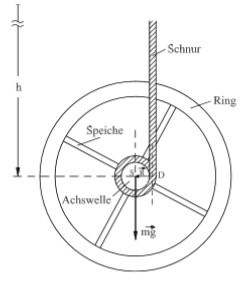
\includegraphics[width=0.5\linewidth]{res/Fallrad}
	\caption{Seitenansicht des maxwellschen Fallrades.\cite{lw}}
	\label{fig:fallrad}
\end{figure}


Aus dem geometrischen Ausbau sowie der Masse folgt das Trägheitsmoment bezüglich des Schwerpunktes, die Beschleunigung konnte direkt bestimmt werden. Der Steinersche Satz erlaubt nun Rückschlüsse auf den Abrollradius. Dieser wurde mit dem gemessenen Radius verglichen.






\subsection{Methoden}
Zur Bestimmung des Trägheitsmomentes wurde das Rad unter Benutzung eines Messschiebers mit Nonius vermessen. Alle Bestandteile wurden hierbei als Voll- oder Hohlzylinder betrachtet. Die Verdickung am Schnittpunkt der Achsen wurde nicht vermessen, zum Ausgleich wurde das Schnittvolumen doppelt berücksichtigt. Da der Abstand der Verdickung zur Drehachse klein gegenüber dem Abstand des äußeren Ringes ist, ist davon auszugehen das der Unterschied zu vernachlässigen ist. Größen welche in vierter Potenz in das Trägheitsmoment eingingen wurden mehrfach gemessen, um den Einfluss von möglichen Unebenheiten des Rades auf die Ergebnisse zu verringern. Die Masse des Rades wurde mittels einer Waage bestimmt.
Anschließend wurden die Fallzeiten $t$ für fünf verschiedene Höhen $h$ je fünfmal mit einer Stoppuhr manuell bestimmt.



%\subsection{Relevante Gleichungen und Zusammenhänge}



%Für die Beschleunigung gilt\\
%$g^*= g \cdot \frac{m R^2}{J_s+m R^2}$\\
%2 Integrieren und umstellen folgt\\
%$\frac{H}{T^2}= \frac{g^*}{2}=c_{Diagramm}$\\
%Das Trägheitsmoment im  Schwerpunkt\\
%$J_s=$\\


%Aus .. folgt für den Abrollradius:\\
%$R=\sqrt{\frac{2cJ_s}{m(g-2c)}}$


\subsection{Daten und Analyse} %Fallrad\begin{figure}
Im Folgenden soll nun zunächst das Trägheitsmoment bezüglich des Schwerpunktes $J_s$ bestimmt werden. Anschließend wird die effektive Beschleunigung aus den Fallzeiten für verschiedene Höhen ermittelt und abschließend werden die Abrollradien mit Hilfe des Steinerschen Satzes verglichen.

\subsubsection{Bestimmung Trägheitsmoment im Schwerpunkt}

Allgemein ist das Trägheitsmoment J definiert durch:
\begin{align}
J= \int_{V} \vec{r}_{\perp} \varrho (\vec{r}) \mathrm{d}V.
\end{align}
Angewandt auf die vorliegende Geometrie bei Annahme einer konstanten Massenverteilung folgt bezüglich der Symmetrieachse folgt: 
\begin{align}
J_s&= J_{K}+2J_{S}+J_{A}\\
&=\varrho \pi \left[\frac{H_K}{2} (R_a^4-R_i^4)+  2 H_S(\frac{H_S^2}{12} R_S^2+\frac{R_S^4}{4})+  \frac{H_A}{2}R_A^4  \right] \label{eq:taddfall}.
\end{align}	
Wobei $H$ die jeweilige Höhe und R den jeweiligen Radius des Zylinders beschreiben. $R_a$ und $R_i$ stehen für Außen- bzw. Innenradius des äußeren Kreisrings. Die Dichte $\varrho$ ist als Masse pro Volumen gegeben mit
\begin{align}
	\varrho=\frac{M}{\pi(H_K  (R_a^2-R_i^2)+2 H_S  R_S^2+ H_A  R_A^2)}. \label{eq:dichtefall}
\end{align} 
Durch Einsetzten der Gleichungen \ref{eq:dichtefall} in Gleichung \ref{eq:taddfall} erhält man das Trägheitsmoment
\begin{align}
J_s=\frac{M \left(2 H_{S} \left(\frac{H_{A} R_{A}^{4}}{2} + \frac{H_{S}^{2} R_{S}^{2}}{12} + \frac{R_{S}^{4}}{4}\right) + \frac{ H_{k}}{2} \left(R_{a}^{4} - R_{i}^{4}\right)\right)}{H_{A} R_{A}^{2} + H_{k} \left(R_{a}^{2} - R_{i}^{2}\right) + 2 R_{S}^{2} R_{i}} \label{eq:Jfall}.
\end{align}
Die Abmessungen welche mehrfach gemessen wurden, wurden arithmetisch gemittelt ihre Unsicherheit wurde nach Gleichung \ref{eq:kombsu} unter Berücksichtigung der Ableseungenauigkeit($\SI{0.02}{mm}$)  und der statistischen Unsicherheit berechnet, die Ergebnisse sind in Tabelle \ref{tab:datafall} notiert.
Mit den Messwerten aus Tabelle \ref{tab:datafall} folgt aus den Gleichungen \ref{eq:Jfall} und \ref{eq:uJfall} bezüglich der Symmetrieachse $J_s=\SI{0.003702 \pm 0.000008}{kg\cdot m^2}$. Der relative Fehler ist $\frac{\Delta J_s}{J_s}=0.2\%$. 



\begin{table}
	\centering
	\caption{Abmessungen des Fallrades}
	\begin{tabular}{|l|c|}
	\hline 
	Masse des Fallrades $M$& \SI{0.732040\pm 0.000006}{kg} \\ 
	\hline 
	Höhe bzw. Tiefe des Kreisrings $H_k$ K& \SI{0.01162\pm 0.00004}{m} \\ 
	\hline 
	Außenradius $R_a$ & \SI{0.08511\pm 0.00003}{m} \\ 
	\hline 
	Innenradius und Speichenhöhe $R_i=H_S$ & \SI{0.07271\pm 0.00004}{m}  \\ 
	\hline 
	Außenradius $R_a$	& \SI{0.00405 \pm 0.00002}{m} \\ 
	\hline 
	Speichenradius $R_S$& \SI{0.00403 \pm 0.00003}{m} \\ 
	\hline 
	Achsenhöhe $H_A$& \SI{0.20030\pm 0.00002}{m} \\ 
	\hline 

\end{tabular}
\label{tab:datafall} 
\end{table}








\subsubsection{Bestimmung der effektiven Beschleunigung }
Um abschließend den gemessenen Abrollradius mit dem Abrollradius nach steinerschem Satz vergleichen zu können, wird neben dem Trägheitsmoment die effektive Beschleunigung $g^*$ benötigt.





\begin{figure}[h!]
	\centering
	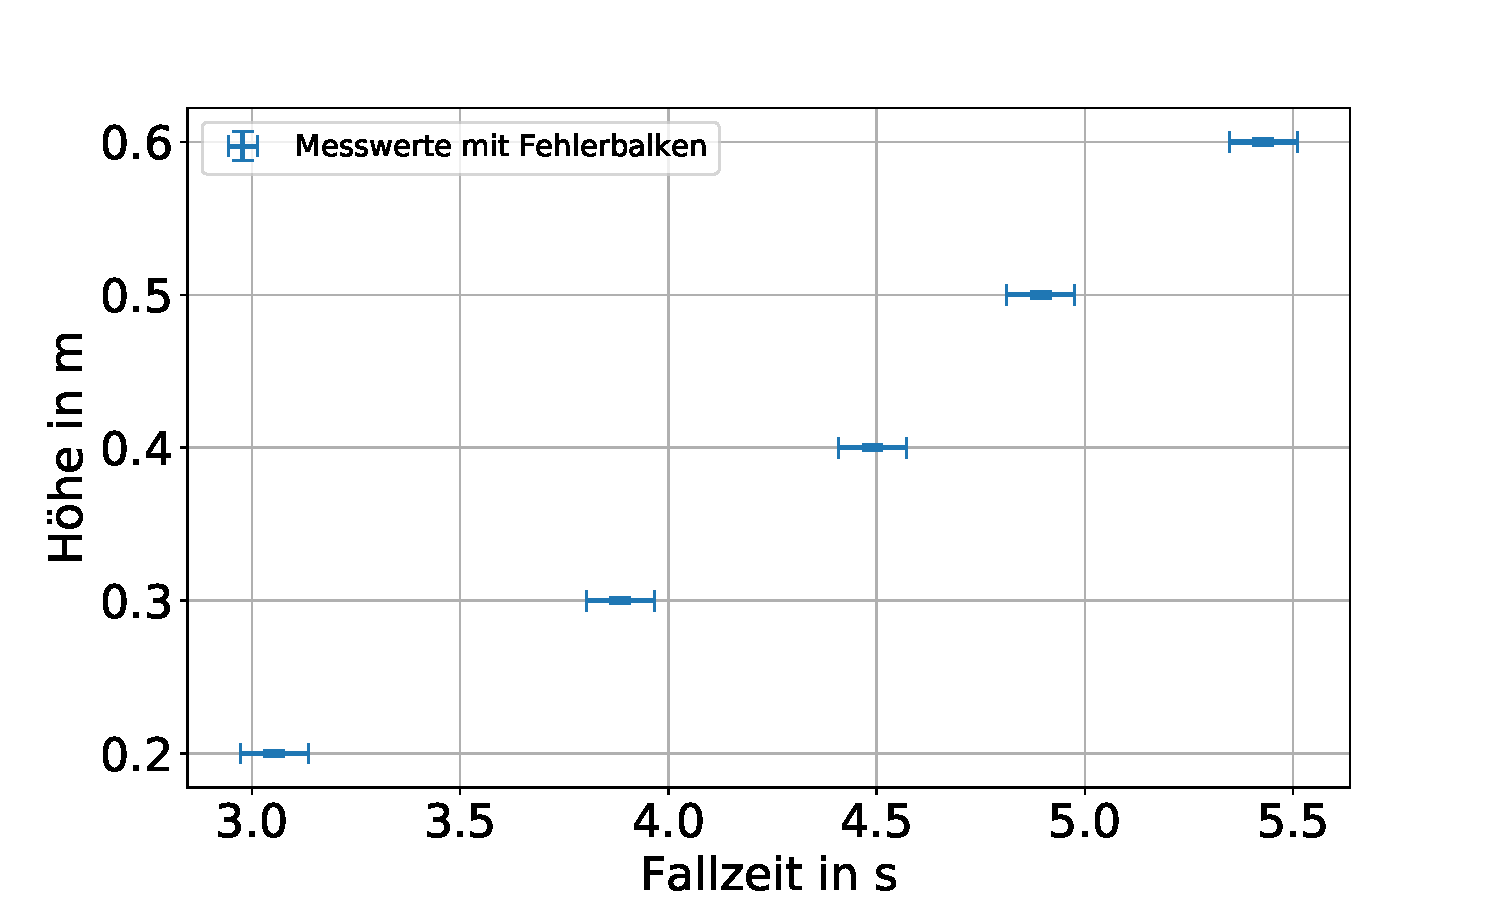
\includegraphics[width=0.7\linewidth]{auswertung/Fallrad/h,t}
	\caption{Die Höhe $h$ des Fallrades in Abhängigkeit der jeweiligen Fallzeiten $t$.}
	\label{fig:ht}
\end{figure}



\begin{figure}[h!]
	\centering
	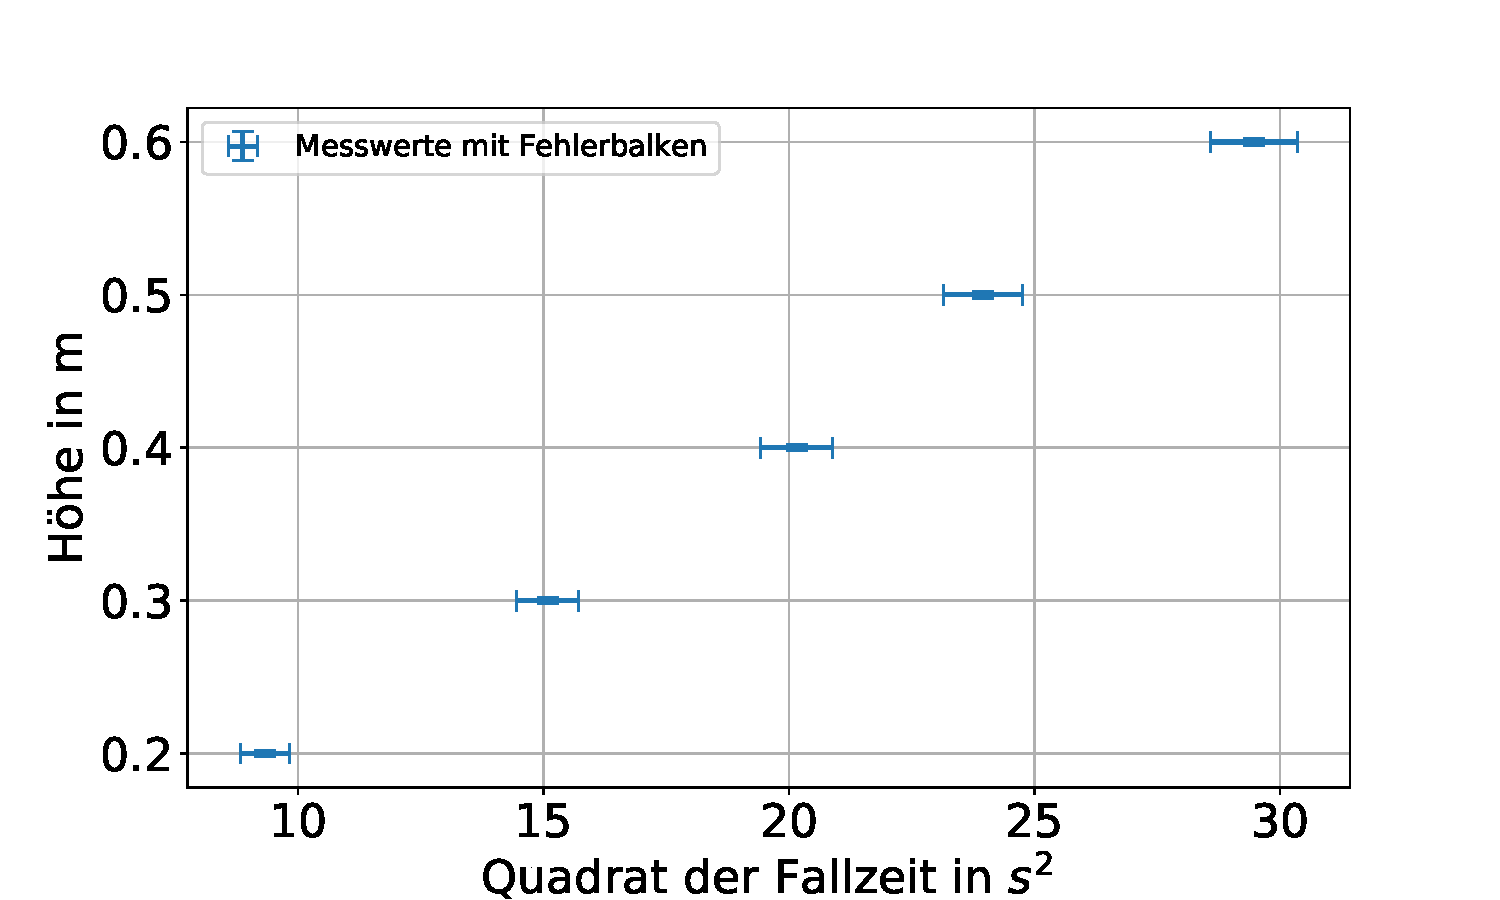
\includegraphics[width=0.7\linewidth]{auswertung/Fallrad/h,t^2}
	\caption{Die Messpunkte nach \cref{fig:ht} in Einheiten von $t^2$. }
	\label{fig:ht2}
\end{figure}

\begin{figure}[h!]
	\centering
	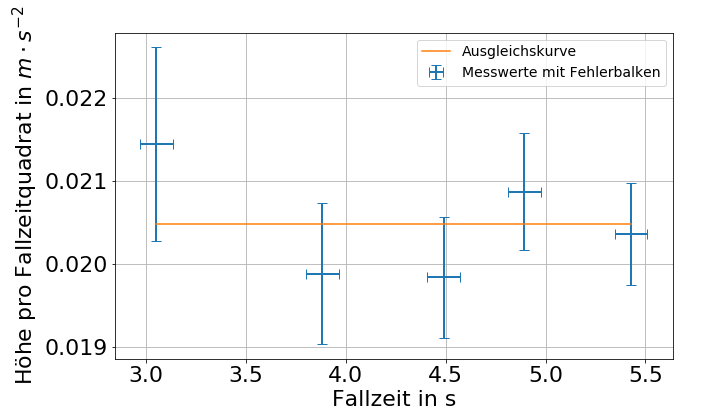
\includegraphics[width=0.7\linewidth]{auswertung/Fallrad/T,ht^-2}
	\caption{Messpunkte aus \cref{fig:ht} in Einheiten von $\frac{h}{t^2}$}
	\label{fig:tht-2}
\end{figure}





Die Abbildung \ref{fig:ht} stellt die Messwerte dar. Da die theoretischen Betrachtungen und der Graph eine quadratische Abhängigkeit suggerieren, werden diese Messwerte anschließend in Abbildung \ref{fig:ht2} linearisiert dargestellt. Abbildung \ref{fig:tht-2} stellt die jeweiligen Steigungen einer geraden durch Ursprung und Messpunkt der Abbildung \ref{fig:ht2} dar. \\






Anschließend wurde das arithmetische Mittel $c$ der Datenpunkte aus Abbildung \ref{fig:tht-2} gebildet. Aus der zugehörigen Bewegungsgleichung ist abzulesen, dass $\frac{g^*}{2}=\frac{h}{T^2}=c$. Es folgt: $g^*=\SI{0.0410 \pm  0.0019}{m \per s \squared}$.





\subsubsection{Vergleich der Abrollradien}


Aus der Zusammenhang zwischen der effektiven Beschleunigung und  dem Abrollradius nach Gleichung \ref{eq:gs} folgt für den Abrollradius Gleichung \ref{eq:R}.

\begin{align}
g^*  &= g \frac{mR^2}{J_s + m R^2}= 2c \label{eq:gs}\\
R&=\sqrt{\frac{2 c J_s}{M (g-2c)}} \label{eq:R}
\end{align}

Mit den Messwerten aus Tabelle \ref{tab:datafall}, der effektiven Beschleunigung $g^*$ aus Abbildung \ref{fig:tht-2} sowie der Fallbeschleunigung g aufgrund des Erdschwerefeldes und der Unsicherheit nach Gleichung \ref{eq:uR} folgt $R=\SI{0.00460\pm 0.00011}{m}$. Die Messung der Durchmesser von Faden und Aufhängeachse mit dem Messschieber ergab einen Radius $R_{geometrisch}=\SI{0.00455 \pm 0.00004}{m}$. Der direkt gemessene Radius bestätigt den zuvor errechneten Wert. Des weiteren liefert die direkte Messung erwartungsgemäß die kleinere Unsicherheit.  
%19

\section{Schlussfolgerung}
Im ersten Teil der Auswertung wurde der Eleatizitätsmodul $E$ bestimmt. Beim Vergleich von den Experimentell bestimmten Werten mit Literaturwerten fiel auf das die Vermutung das es sich bei der Messingfarbenden Runden Stange um Messing handelte vermutlich falsch ist, da die Werte für den Elastizitätsmodul 
























Das Torsionspendel eignete sich um den Schubmodul( $G =\SI{7.87+-0.09e10}{kg \per \second \squared  \metre}$) des verwendeten Drahtes bei bekanntem Trägheitsmoment zu bestimmen und durch diese Materialeigenschaft Rückschlüsse auf das verwendete Material (Stahllegierung) zu ziehen. Da der Schubmodul jedoch von dem Fertigungsprozess und den Beimengungen abhängt, ist dies nur als Richtwert zu verstehen. Bei bekanntem Schubmodul $G$ und den Abmessungen des Drahtes bzw. dem Direktionsmodul $D^*=\SI{8.2+-0.2e-5}{\kilogram \metre \squared \per \second \squared }$  lässt sich aus der Schwingungsdauer das jeweilige Trägheitsmoment berechnen.  Die gemessenen  Trägheitsmoment  sind \cref{tab:vglJ} zu entnehmen.











% --- Anhang einbinden
\IfFileExists{tex/20_Anhang.tex}{
	\clearpage
	\appendix
	\section{Anhang}
	\label{sec:anhang}
	

\subsection{Verwendete Gleichungen}\label{VGuD}
%und Definition der Variablen


%Zusammenhang zwischen Kreisfrequenz $\omega$ und Schwingungsdauer $T$:

%\begin{align}
%	T=\frac{2 \pi}{\omega} \pm \Delta t
%	\label{eq:T}
%\end{align} 


%Alle anderen Unsicherheiten sind gemäß Kapitel \ref{sec:einzeln} so klein, dass sie zu vernachlässigen sind. Es sei $\Delta t={ 0,006} {s}$.\\
%\frac{2 \pi}{\omega^2} \cdot\Delta \omega  \label{eq:T}


%Standardunsicherheit der Rechteckverteilung u für die Intervallbreite a:
	%\begin{align}
	%	u=\frac{a}{2\sqrt{3}}\label{eq:SR}
	%\end{align} 



}{}

% --- Literaturverzeichnis mit BibLaTeX
\ifthenelse{\boolean{showBibliography}}{
	%\clearpage
	\printbibliography
}{}

\end{document}

